\documentclass[11pt,a4paper]{article}

\usepackage[margin=2.4cm]{geometry}
\usepackage{fontspec}
\usepackage{microtype}
\usepackage{xcolor}
\usepackage{listings}
\usepackage{booktabs}
\usepackage{tabularx}
\usepackage{enumitem}
\usepackage{tikz}
\usetikzlibrary{positioning,arrows.meta,fit,backgrounds}
\usepackage[hidelinks]{hyperref}


\definecolor{codebg}{HTML}{F6F8FA}
\definecolor{outbg}{HTML}{FFFFFF}
\definecolor{rule}{HTML}{D0D7DE}
\definecolor{kw}{HTML}{0550AE}
\definecolor{str}{HTML}{0A3069}
\definecolor{com}{HTML}{6E7781}
\definecolor{accent}{HTML}{1F6F8B}
\definecolor{warn}{HTML}{9A6700}

\lstdefinestyle{py}{
  language=Python,
  basicstyle=\ttfamily\small,
  keywordstyle=\color{kw}\bfseries,
  stringstyle=\color{str},
  commentstyle=\color{com}\itshape,
  backgroundcolor=\color{codebg},
  frame=single,
  rulecolor=\color{rule},
  framesep=4pt,
  xleftmargin=6pt,
  xrightmargin=6pt,
  showstringspaces=false,
  columns=fullflexible,
  keepspaces=true,
  breaklines=true,
  breakatwhitespace=true,
  aboveskip=8pt,
  belowskip=4pt,
  morekeywords={with,as,assert,None,True,False,self},
  deletecomment=[s]{"""}{"""},
  morestring=[s]{"""}{"""},
}
\lstdefinestyle{out}{
  basicstyle=\ttfamily\footnotesize,
  backgroundcolor=\color{outbg},
  frame=leftline,
  rulecolor=\color{accent},
  framerule=1.5pt,
  xleftmargin=10pt,
  columns=fixed,
  keepspaces=true,
  breaklines=true,
  aboveskip=2pt,
  belowskip=10pt,
}
\lstdefinestyle{sql}{
  style=py,
  language=SQL,
  morekeywords={MERGE,USING,MATCHED,ATTACH,READ_ONLY,BIGINT},
}
\lstnewenvironment{python}{\lstset{style=py}}{}
\lstnewenvironment{console}{\lstset{style=out}}{}
\lstnewenvironment{sqlcode}{\lstset{style=sql}}{}
\newcommand{\code}[1]{\texttt{#1}}

\newenvironment{note}[1][Note]
  {\par\smallskip\noindent\begin{minipage}{\linewidth}\color{black}%
   \hrule height 0.6pt\relax\vspace{4pt}\textbf{\color{accent}#1.}\ }
  {\vspace{4pt}\hrule height 0.6pt\end{minipage}\par\smallskip}

\setlist{itemsep=2pt,topsep=4pt}
\setlength{\emergencystretch}{3em}

\title{\textbf{ducktide}\\[4pt]\large Immutable Pydantic models and append-fast time series on DuckDB and Polars}
\author{Thomas Schmelzer}
\date{Version 0.1.0 \quad September 2026}

\begin{document}
\maketitle

\begin{abstract}
\noindent
ducktide is a small persistence layer for Python. It stores two kinds of data:
\emph{reference data} (instruments, sensors, accounts) as frozen Pydantic models in
relational tables, and \emph{time series} (prices, volumes, readings) as columnar tables
written by idempotent bulk upserts and read back as Polars DataFrames. Both run on DuckDB,
in memory or in a single file, with no server and no ORM framework. This document
introduces the library, explains the design decisions behind it, and works through its
API with examples. Every example was run against ducktide 0.1.0, and the output shown is
what it printed.
\end{abstract}

\tableofcontents
\bigskip

% ---------------------------------------------------------------------------
\section{Introduction}

A great deal of analytical code has the same persistence needs. There is a modest set
of \emph{things}: financial instruments, sensors, customers. Each has a handful of
attributes and changes rarely. And there is a large volume of \emph{measurements} about
those things, arriving continuously, occasionally late, sometimes corrected after the
fact. A research notebook, a nightly ingest job and a backtest all want to read both, and
none of them wants to run a database server.

DuckDB already solves the hard part. It is an embedded, columnar SQL engine that runs
inside the Python process, stores a whole database in one file, reads and writes Parquet
and CSV natively, and hands query results to Polars without copying them. ducktide does
not replace any of that. It is candy on top of the DuckDB cake: a thin, opinionated layer
that turns a few hundred lines of SQL you would otherwise write, and get subtly wrong, into
a small API.

What the layer adds:

\begin{itemize}
  \item \textbf{One definition per table.} A Pydantic model \emph{is} the schema. Column
    names, DuckDB types and \code{NOT NULL} constraints are derived from its fields.
  \item \textbf{Typed values back.} Entity reads return validated, frozen model instances,
    never tuples.
  \item \textbf{Correct upserts.} Time-series ingestion merges on a series key, so
    re-ingesting overlapping data is safe and corrections and late rows land.
  \item \textbf{Performance traps avoided.} Bulk inserts go through one frame instead of
    row-by-row statements, fragmented frames are rechunked before ingest, and tables can
    be compacted by series key.
  \item \textbf{Safe SQL.} Identifiers are validated and quoted in one module, and values
    always travel as bound parameters.
\end{itemize}

When you need something the layer does not cover, the DuckDB connection is right there,
and plain SQL works on the same tables.

\subsection{Installation}

\begin{console}
pip install ducktide        # or: uv add ducktide
\end{console}

ducktide requires Python 3.11 or later. Its runtime dependencies are DuckDB, Polars,
Pydantic and PyArrow (used by DuckDB to hand results to Polars).

\subsection{A first look}

The shortest useful program defines a model, attaches it to a database and reads it
back:

\begin{python}
from ducktide import DB, DomainModel, Table

class Sensor(DomainModel):
    id: int
    name: str
    site: str

db = DB(tables_map={"sensor": Table.of(Sensor)})   # in memory
db.sensor.insert(Sensor(id=1, name="north", site="berlin"))
db.sensor.get(1)
\end{python}
\begin{console}
Sensor(id=1, name='north', site='berlin')
\end{console}

The time-series half is just as short. The table is created on the first ingest:

\begin{python}
from datetime import datetime
import polars as pl
from ducktide import TimeSeriesDB

ts = TimeSeriesDB()                                   # or TimeSeriesDB("prices.duckdb")
ts.ingest("prices", pl.DataFrame({
    "timestamp": [datetime(2025, 1, 2), datetime(2025, 1, 3)],
    "instrument_id": [1, 1],
    "close": [100.0, 101.0],
}))
ts.get_timeseries_frame("prices", instrument_id=1)    # a polars.DataFrame
\end{python}

% ---------------------------------------------------------------------------
\section{Design}

\subsection{Two stores, one engine}

ducktide has two entry points, \code{DB} and \code{TimeSeriesDB}. They are split by the
\emph{shape} of the data and by how it is read and written, not by storage engine:
both are DuckDB. Table~\ref{tab:two} contrasts them.

\begin{table}[h]
\centering\small
\begin{tabularx}{\linewidth}{@{}l X X@{}}
\toprule
 & \textbf{Reference data} (\code{DB} + \code{Table}) & \textbf{Time series} (\code{TimeSeriesDB}) \\
\midrule
Examples      & instruments, exchanges, sensors & prices, volumes, readings \\
Volume        & hundreds to thousands of rows   & millions of rows \\
Identity      & a primary key                   & series key plus timestamp \\
Schema        & declared by a Pydantic model    & taken from the first frame ingested \\
Writes        & inserts of validated objects    & bulk upserts (\code{MERGE}) \\
Reads         & frozen model instances          & Polars DataFrames, sorted by time \\
Tuning        & none needed                     & physical row order (\code{compact}) \\
\bottomrule
\end{tabularx}
\caption{The two halves of ducktide.}
\label{tab:two}
\end{table}

Forcing both into one abstraction would hurt one of them. Row objects make time series
slow: building a million Pydantic instances takes seconds and a great deal of memory for
what Polars returns in milliseconds. Bare frames, in turn, would cost reference data its
validation and types.

Keeping the two in separate files pays off operationally too:

\begin{itemize}
  \item \textbf{Writers do not block each other.} DuckDB permits one read-write process
    per file. A nightly price ingest holding the time-series file does not lock the
    instrument table.
  \item \textbf{Different lifecycles.} Reference data is small and worth backing up or
    versioning. Time series are large, can usually be re-downloaded from a vendor, and can
    be rebuilt without touching the definitions.
  \item \textbf{Read-only fan-out.} Many processes can open the time-series file with
    \code{read\_only=True} while the reference database stays writable.
\end{itemize}

\code{TimeSeriesModel} connects the two: a model stored in \code{DB} knows its
time-series table and its \code{instrument\_id}, and can fetch or ingest its own series
(Section~\ref{sec:bridge}). Figure~\ref{fig:arch} shows the pieces.

\begin{figure}[h]
\centering
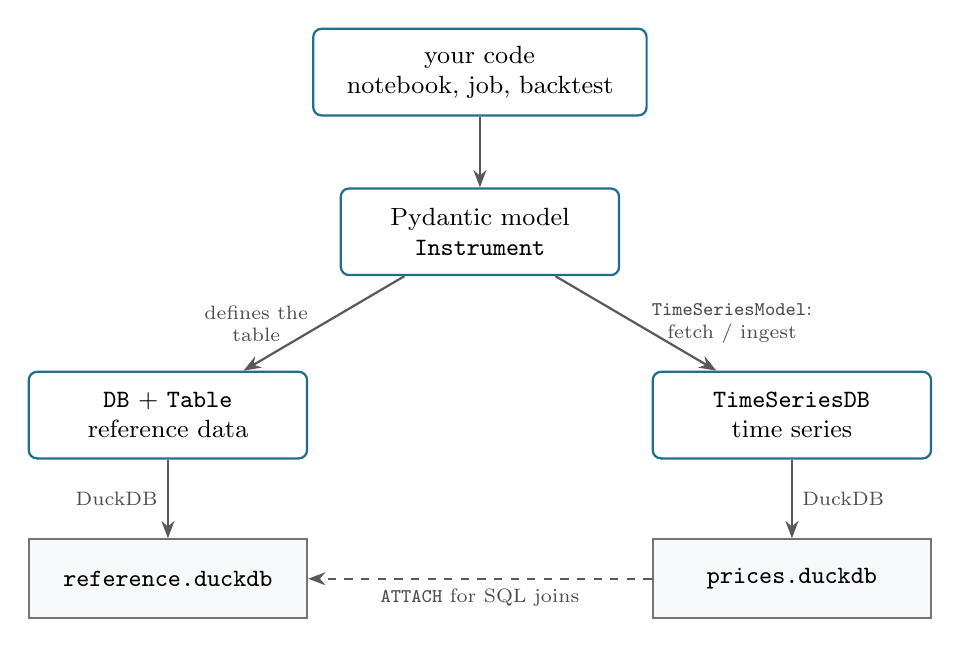
\begin{tikzpicture}[
  box/.style={draw=accent, rounded corners=3pt, thick, align=center, minimum height=11mm, text width=33mm, fill=white, font=\small},
  file/.style={draw=black!55, thick, align=center, minimum height=10mm, text width=33mm, fill=codebg, font=\small\ttfamily},
  arr/.style={-{Stealth[length=2.2mm]}, thick, color=black!65},
  lbl/.style={font=\scriptsize, color=black!70, align=center}
]
\node[box] (model) {Pydantic model\\\code{Instrument}};
\node[box, below left=12mm and 4mm of model] (db) {\code{DB} + \code{Table}\\reference data};
\node[box, below right=12mm and 4mm of model] (ts) {\code{TimeSeriesDB}\\time series};
\node[file, below=10mm of db] (f1) {reference.duckdb};
\node[file, below=10mm of ts] (f2) {prices.duckdb};
\node[box, above=9mm of model, text width=40mm] (app) {your code\\notebook, job, backtest};

\draw[arr] (model) -- node[lbl, left, xshift=-2pt] {defines the\\table} (db);
\draw[arr] (model) -- node[lbl, right, xshift=2pt] {\code{TimeSeriesModel}:\\fetch / ingest} (ts);
\draw[arr] (db) -- node[lbl, left] {DuckDB} (f1);
\draw[arr] (ts) -- node[lbl, right] {DuckDB} (f2);
\draw[arr] (app) -- (model);
\draw[arr, dashed] (f2.west) -- node[lbl, below] {\code{ATTACH} for SQL joins} (f1.east);
\end{tikzpicture}
\caption{Architecture. One model describes a reference table and links to its series. Each store owns one DuckDB file.}
\label{fig:arch}
\end{figure}

\subsection{One model, one table}

A ducktide table is described by exactly one Pydantic model. Its fields \emph{are} the
columns, in declaration order. There is no second ``ORM class'' and no hand-written
\code{CREATE TABLE} to keep in step with it. The mapping from Python types to DuckDB types
is deliberately small and exact (Table~\ref{tab:types}). The lookup is on the exact type,
so \code{bool} never falls through to \code{int} and \code{datetime} never to \code{date}.

\begin{table}[h]
\centering\small
\begin{tabular}{@{}ll@{\qquad}ll@{}}
\toprule
Python & DuckDB & Python & DuckDB \\
\midrule
\code{bool}     & \code{BOOLEAN}   & \code{date}      & \code{DATE} \\
\code{int}      & \code{BIGINT}    & \code{datetime}  & \code{TIMESTAMP} \\
\code{float}    & \code{DOUBLE}    & \code{time}      & \code{TIME} \\
\code{str}      & \code{VARCHAR}   & \code{timedelta} & \code{INTERVAL} \\
\code{bytes}    & \code{BLOB}      & \code{UUID}      & \code{UUID} \\
\code{Decimal}  & \code{DECIMAL}   &                  & \\
\bottomrule
\end{tabular}
\caption{Type mapping used by \code{column\_definitions}.}
\label{tab:types}
\end{table}

Three rules complete the derivation:
\begin{enumerate}
  \item A field annotated \code{X | None} is nullable. Every other field is \code{NOT NULL}.
  \item The primary-key field (default \code{id}) gets \code{PRIMARY KEY}.
  \item \code{sql\_types=\{column: definition\}} replaces a column's derived definition
    wholesale, constraints included. It covers anything the mapping cannot express:
    \code{UNIQUE}, a \code{DECIMAL} precision, or a type outside the table.
\end{enumerate}

\subsection{Values, not active records}

Models carry no \code{save()}, \code{find()} or \code{delete()}. All persistence goes
through a \code{Table}, the repository. Domain objects stay plain values that can be
created in a test, passed between threads, hashed and compared, without dragging a
connection along.

The optional base class \code{DomainModel} fixes the configuration ducktide recommends:
\code{frozen=True}, so a row read back is never mutated behind the table's back, and
stripping of surrounding whitespace from strings (\code{str\_strip\_whitespace=True}). Any Pydantic model can back a table; \code{DomainModel}
is a convenience, not a requirement.

\subsection{Upsert semantics for time series}

A time-series row is identified by its \emph{key}: the series columns plus the timestamp.
By default the series column is \code{instrument\_id} when the frame has one, and there
are no series columns otherwise (a single series). \code{ingest} turns a frame into one
DuckDB \code{MERGE} on that key:

\begin{itemize}
  \item a row whose key is already stored \textbf{replaces} it (a correction);
  \item every other row is \textbf{inserted}, whatever its timestamp (a late row lands
    in the past rather than being dropped);
  \item within one frame, the \textbf{last row for a key wins};
  \item a \code{NULL} key value matches a stored \code{NULL} instead of creating a duplicate;
  \item with \code{on\_conflict="ignore"}, stored rows are kept and only new keys are added.
\end{itemize}

Ingest is therefore \emph{idempotent}: re-running yesterday's job, or ingesting a
window that overlaps what is stored, leaves the table correct. That property is what makes
retries and backfills boring, which is the point.

\subsection{Physical layout}

DuckDB stores rows in blocks and keeps each block's minimum and maximum per column, so it
can skip blocks that cannot match a filter. Ingestion appends in arrival order. When whole
days arrive for every instrument at once, each instrument is spread across the whole
table, and a read for one instrument has to touch nearly every block. \code{compact}
rewrites a table sorted by series key, then timestamp. It is a trade-off, not a free
speed-up (Table~\ref{tab:compact}, one million daily bars for 500 instruments).

\begin{table}[h]
\centering\small
\begin{tabular}{@{}lrr@{}}
\toprule
Read & time order & compacted \\
\midrule
one instrument, one year        & 1.1 ms  & 0.75 ms \\
one day, all instruments        & 0.3 ms  & 1.4 ms \\
mean per instrument, whole table & 0.65 ms & 0.9 ms \\
\bottomrule
\end{tabular}
\caption{Effect of \code{compact} on read latency.}
\label{tab:compact}
\end{table}

Compact only if reads for single series dominate. A table loaded one instrument at a
time is already grouped and gains nothing. New ingests land unsorted again, so compact
periodically, for example after each day's ingest.

\subsection{Safety}

All SQL containing identifiers is composed in one module, \code{ducktide.utils.sql}.
Table, schema and column names pass through \code{validate\_identifier} and
\code{quote\_identifier} before they reach a statement. Keyword filters are checked against
the table's columns, and every data value is a bound parameter. The raw escape hatches
(\code{select(where\_clause, where\_params)}, \code{TimeSeriesDB.query}) take \code{?}
placeholders. Use them, and never format values into SQL strings.

\subsection{Errors}

Every ducktide exception derives from \code{DucktideError}:

\begin{console}
DucktideError
 +-- ValidationError          bad identifier, unknown filter, missing key column
 +-- DataError                data processing or type problems
 +-- DatabaseError
      +-- DatabaseConnectionError
      +-- QueryError          constraint violations, failed time-series reads
\end{console}

Lookups that find nothing raise \code{KeyError}, as a mapping would. Reading a time-series
table that does not exist returns an empty DataFrame: a missing table means ``no data
yet'', not an error.

% ---------------------------------------------------------------------------
\section{Entity tables in practice}

\subsection{Defining and inspecting a table}

\code{column\_definitions} shows exactly what ducktide will create:

\begin{python}
from datetime import date
from ducktide import DB, DomainModel, Table
from ducktide.model import column_definitions

class Sensor(DomainModel):
    id: int
    name: str
    site: str
    installed: date | None = None

column_definitions(Sensor)
\end{python}
\begin{console}
{'id': 'BIGINT PRIMARY KEY', 'name': 'VARCHAR NOT NULL',
 'site': 'VARCHAR NOT NULL', 'installed': 'DATE'}
\end{console}

\begin{python}
column_definitions(Sensor, sql_types={"name": "VARCHAR NOT NULL UNIQUE"})
\end{python}
\begin{console}
{'id': 'BIGINT PRIMARY KEY', 'name': 'VARCHAR NOT NULL UNIQUE',
 'site': 'VARCHAR NOT NULL', 'installed': 'DATE'}
\end{console}

Tables are attached to a \code{DB} through \code{tables\_map}. Each key becomes an
attribute of the database, and \code{db.table} maps model classes to their tables:

\begin{python}
db = DB(tables_map={"sensor": Table.of(Sensor)})      # or db_path="sensors.duckdb"
db.table[Sensor] is db.sensor
\end{python}
\begin{console}
True
\end{console}

\code{Table.of} takes three options: \code{name=} (default: the lower-cased class name),
\code{primary\_key=} (default \code{"id"}) and \code{sql\_types=}. The table is created with
\code{CREATE TABLE IF NOT EXISTS}, so opening an existing file is harmless.

\subsection{Writing}

\begin{python}
db.sensor.insert(Sensor(id=1, name="north", site="berlin", installed=date(2024, 3, 1)))
db.sensor.bulk_insert([
    Sensor(id=2, name="south", site="zurich"),
    Sensor(id=3, name="east", site="berlin", installed=date(2025, 6, 15)),
])
len(db.sensor)
\end{python}
\begin{console}
3
\end{console}

\code{insert(*objs)} takes one or more objects, and delegates to \code{bulk\_insert} for
more than one. \code{bulk\_insert} accepts any iterable and hands DuckDB a single frame
instead of running one statement per row. Use it for anything beyond a handful of objects.
\code{DB.insert(*objs)} routes each object to its model's table, which is convenient when a
batch mixes models.

Constraint violations surface as \code{QueryError}:

\begin{python}
from ducktide.exceptions import QueryError

try:
    db.sensor.insert(Sensor(id=1, name="dup", site="x"))
except QueryError as exc:
    print(exc)
\end{python}
\begin{console}
Constraint violation inserting into 'sensor': Constraint Error: Duplicate key "id: 1"
violates primary key constraint.
\end{console}

\subsection{Reading}

Point lookups by primary key or by any column:

\begin{python}
db.sensor.get(2)
db.sensor[3].name
db.sensor.get_by("name", "east")
\end{python}
\begin{console}
Sensor(id=2, name='south', site='zurich', installed=None)
'east'
Sensor(id=3, name='east', site='berlin', installed=datetime.date(2025, 6, 15))
\end{console}

All three raise \code{KeyError} when no row matches (\code{get(None)} returns \code{None}).

\code{select} filters with keyword arguments. A bare column name tests equality, and
\code{None} tests for SQL \code{NULL}. The suffixes \code{\_before} ($<$), \code{\_after}
($>$), \code{\_at\_or\_before} ($\le$) and \code{\_at\_or\_after} ($\ge$) express ranges.
Several filters combine with \code{AND}:

\begin{python}
[s.id for s in db.sensor.select(site="berlin")]
[s.id for s in db.sensor.select(installed=None)]
[s.id for s in db.sensor.select(installed_after=date(2025, 1, 1))]
[s.id for s in db.sensor.select(site="berlin", id_at_or_before=2)]
\end{python}
\begin{console}
[1, 3]
[2]
[3]
[1]
\end{console}

Filter names are validated against the table, so a typo fails loudly:

\begin{python}
db.sensor.select(colour="red")
\end{python}
\begin{console}
ValidationError: Unknown filter 'colour' for table 'sensor'. Valid columns: id, name,
site, installed. Comparison suffixes: _after, _at_or_after, _at_or_before, _before
\end{console}

For anything keywords cannot express, pass a raw \code{WHERE} clause with placeholders.
It is appended last, so \code{ORDER BY} and \code{LIMIT} work:

\begin{python}
[s.name for s in db.sensor.select("site = ? ORDER BY name", ["berlin"])]
\end{python}
\begin{console}
['east', 'north']
\end{console}

A table is also a small collection: \code{len(table)}, \code{bool(table)},
\code{iter(table)}, and the properties \code{exists} and \code{empty}.

\subsection{Values are immutable}

Rows come back frozen. To change one, derive a new value and write it:

\begin{python}
s = db.sensor.get(1)
s.site = "paris"                                   # raises pydantic ValidationError
moved = s.model_copy(update={"site": "paris"})
\end{python}
\begin{console}
Sensor(id=1, name='north', site='paris', installed=datetime.date(2024, 3, 1))
\end{console}

\code{Table} has no update or delete method yet. Both are one statement through the
connection:

\begin{python}
db.execute_query("UPDATE sensor SET site = ? WHERE id = ?", ["paris", 1])
db.execute_query("DELETE FROM sensor WHERE id = ?", [2])
[(x.id, x.site) for x in db.sensor]
\end{python}
\begin{console}
[(1, 'paris'), (3, 'berlin')]
\end{console}

\code{Table.execute(sql, params)} runs a query and reads the rows back as models, which is
the way to use SQL that \code{select} cannot express while still getting typed values:

\begin{python}
db.sensor.execute("SELECT * FROM sensor WHERE site = ?", ["paris"])
\end{python}
\begin{console}
[Sensor(id=1, name='north', site='paris', installed=datetime.date(2024, 3, 1))]
\end{console}

\subsection{A model with a non-default key and exact decimals}

\begin{python}
from datetime import datetime
from decimal import Decimal

class Trade(DomainModel):
    trade_id: int
    ticker: str
    qty: int
    price: Decimal
    executed_at: datetime

column_definitions(Trade)          # fails: there is no field called id
\end{python}
\begin{console}
ValidationError: Trade has no field(s) id
\end{console}

\begin{python}
trades = Table.of(Trade, name="trades", primary_key="trade_id",
                  sql_types={"price": "DECIMAL(18, 6) NOT NULL"})
db2 = DB(tables_map={"trades": trades})
db2.trades.insert(Trade(trade_id=7, ticker="ACME", qty=100,
                        price=Decimal("101.25"), executed_at=datetime(2025, 1, 2, 14, 30)))
db2.trades.get_by("trade_id", 7)
\end{python}
\begin{console}
Trade(trade_id=7, ticker='ACME', qty=100, price=Decimal('101.250000'),
      executed_at=datetime.datetime(2025, 1, 2, 14, 30))
\end{console}

Note that \code{get} looks up the configured primary key, so \code{db2.trades.get(7)} works
too.

\subsection{Frames, Parquet and CSV}

\begin{python}
db.sensor.to_frame()
\end{python}
\begin{console}
| id | name  | site   | installed  |
|----|-------|--------|------------|
| 1  | north | berlin | 2024-03-01 |
| 2  | south | zurich | null       |
| 3  | east  | berlin | 2025-06-15 |
\end{console}

\code{to\_parquet(path)} and \code{to\_csv(path, delimiter=",", header=True, overwrite=True)}
export through DuckDB's native writers. \code{from\_parquet(path)} and
\code{from\_csv(path)} append a file's rows to the table and return how many they
imported. The file must match the table's columns. Paths are validated before they reach
SQL.

\begin{python}
db.sensor.to_parquet("sensors.parquet")      # the parent folder must exist

fresh = DB(tables_map={"sensor": Table.of(Sensor)})
fresh.sensor.from_parquet("sensors.parquet")
\end{python}
\begin{console}
3
\end{console}

% ---------------------------------------------------------------------------
\section{Time series in practice}

\subsection{Ingest, correct, backfill}

\begin{python}
from datetime import date, datetime
import polars as pl
from ducktide import TimeSeriesDB

ts = TimeSeriesDB()
ts.ingest("prices", pl.DataFrame({
    "timestamp": [datetime(2025, 1, 2), datetime(2025, 1, 3)] * 2,
    "instrument_id": [1, 1, 2, 2],
    "close": [100.0, 101.0, 50.0, 49.5],
}))
ts.tables(), ts.has_table("prices")
\end{python}
\begin{console}
(['prices'], True)
\end{console}

The table was created from the frame's schema. The next frame carries a correction for
3 January and a late bar from the previous year. Both land:

\begin{python}
ts.ingest("prices", pl.DataFrame({
    "timestamp": [datetime(2025, 1, 3), datetime(2024, 12, 31)],
    "instrument_id": [1, 1],
    "close": [101.2, 99.0],
}))
ts.get_timeseries_frame("prices", instrument_id=1)
\end{python}
\begin{console}
| timestamp           | instrument_id | close |
|---------------------|---------------|-------|
| 2024-12-31 00:00:00 | 1             | 99.0  |
| 2025-01-02 00:00:00 | 1             | 100.0 |
| 2025-01-03 00:00:00 | 1             | 101.2 |
\end{console}

With \code{on\_conflict="ignore"}, stored rows win and only new keys are added. That suits
a source you trust less than what is already stored:

\begin{python}
ts.ingest("prices", pl.DataFrame({
    "timestamp": [datetime(2025, 1, 3), datetime(2025, 1, 6)],
    "instrument_id": [1, 1],
    "close": [0.0, 102.0],
}), on_conflict="ignore")
ts.get_timeseries_frame("prices", instrument_id=1)["close"].to_list()
\end{python}
\begin{console}
[99.0, 100.0, 101.2, 102.0]
\end{console}

Duplicate keys inside one frame collapse to the last row:

\begin{python}
ts.ingest("prices", pl.DataFrame({
    "timestamp": [datetime(2025, 1, 7)] * 2,
    "instrument_id": [2, 2],
    "close": [48.0, 48.1],
}))
ts.get_timeseries_frame("prices", instrument_id=2)["close"].to_list()
\end{python}
\begin{console}
[50.0, 49.5, 48.1]
\end{console}

A frame without the timestamp or key columns is rejected before anything is written:

\begin{python}
ts.ingest("prices", pl.DataFrame({"close": [1.0]}))
\end{python}
\begin{console}
ValidationError: frame is missing key column(s): timestamp
\end{console}

\subsection{Reading}

\code{get\_timeseries\_frame} takes the table and the optional filters
\code{instrument\_id}, \code{start}, \code{end} and \code{timezone}. It returns a frame sorted by time, flagged as sorted for Polars. Both bounds
are inclusive. A missing table yields an empty frame.

\begin{python}
ts.get_timeseries_frame("prices", start=date(2025, 1, 3), end=date(2025, 1, 6)).height
ts.get_timeseries_frame("missing").shape
\end{python}
\begin{console}
3
(0, 0)
\end{console}

For SQL beyond these filters, \code{query(sql, *args)} returns a Polars frame. Values are
passed positionally for the \code{?} placeholders:

\begin{python}
ts.query("""
    SELECT instrument_id, avg(close) AS mean_close, count(*) AS n
    FROM prices GROUP BY instrument_id ORDER BY instrument_id
""")
ts.query("SELECT * FROM prices WHERE close > ? ORDER BY timestamp", 100.0).height
\end{python}
\begin{console}
| instrument_id | mean_close | n |
|---------------|------------|---|
| 1             | 100.55     | 4 |
| 2             | 49.2       | 3 |
2
\end{console}

\subsection{Other series keys and schemas}

Series need not be keyed by \code{instrument\_id}. Pass \code{key=} with the columns
identifying one series (the timestamp is added automatically). Table names may be
schema-qualified. A missing schema is created on first ingest.

\begin{python}
fx = pl.DataFrame({
    "timestamp": [datetime(2025, 1, 2)] * 2,
    "base": ["EUR", "GBP"], "quote": ["USD", "USD"], "rate": [1.035, 1.24],
})
ts.ingest("market.fx", fx, key=["base", "quote"])
ts.ingest("market.fx", pl.DataFrame({
    "timestamp": [datetime(2025, 1, 2)], "base": ["EUR"], "quote": ["USD"], "rate": [1.036],
}), key=["base", "quote"])
ts.query("SELECT base, quote, rate FROM market.fx ORDER BY base")
\end{python}
\begin{console}
| base | quote | rate  |
|------|-------|-------|
| EUR  | USD   | 1.036 |
| GBP  | USD   | 1.24  |
\end{console}

The timestamp column is called \code{timestamp} unless configured otherwise:

\begin{python}
sensors = TimeSeriesDB(time_col="ts")
sensors.ingest("readings", pl.DataFrame({
    "ts": [datetime(2025, 1, 1, 0, 0), datetime(2025, 1, 1, 0, 5)],
    "sensor_id": [3, 3],
    "celsius": [4.1, 4.3],
}), key=["sensor_id"])
sensors.get_timeseries_frame("readings")
\end{python}
\begin{console}
| ts                  | sensor_id | celsius |
|---------------------|-----------|---------|
| 2025-01-01 00:00:00 | 3         | 4.1     |
| 2025-01-01 00:05:00 | 3         | 4.3     |
\end{console}

\subsection{Time zones}

Store timezone-aware timestamps as UTC and convert on the way out with \code{timezone=}:

\begin{python}
tz = TimeSeriesDB()
tz.ingest("ticks", pl.DataFrame({
    "timestamp": [datetime(2025, 1, 2, 14, 30)], "px": [1.0],
}).with_columns(pl.col("timestamp").dt.replace_time_zone("UTC")))
tz.get_timeseries_frame("ticks", timezone="America/New_York")
\end{python}
\begin{console}
| timestamp               | px  |
|-------------------------|-----|
| 2025-01-02 09:30:00 EST | 1.0 |
\end{console}

\subsection{Compaction, Parquet and CSV}

\begin{python}
ts.compact("prices")                           # grouped by instrument_id, then time
ts.compact("market.fx", key=["base", "quote"])

ts.export_parquet("prices", "prices.parquet")
archive = TimeSeriesDB()
archive.import_parquet("prices.parquet", "prices")
archive.get_timeseries_frame("prices").height
\end{python}
\begin{console}
7
\end{console}

\code{export\_csv} and \code{import\_csv} work the same way. \code{TimeSeriesDB} is a
context manager that closes its connection on exit:

\begin{python}
with TimeSeriesDB("prices.duckdb") as store:
    latest = store.query("SELECT max(timestamp) AS t FROM prices")
\end{python}

\subsection{Analysis with Polars}

The frame that comes back is ordinary Polars, so analysis starts immediately:

\begin{python}
daily = TimeSeriesDB()
daily.ingest("daily", pl.DataFrame({
    "timestamp": [datetime(2025, 1, d) for d in (2, 3, 6, 7, 8)],
    "instrument_id": [1] * 5,
    "close": [100.0, 102.0, 101.0, 104.0, 103.0],
}))
daily.get_timeseries_frame("daily", instrument_id=1).with_columns(
    ret=pl.col("close").pct_change(),
    ma3=pl.col("close").rolling_mean(3),
).select("timestamp", "close", "ret", "ma3")
\end{python}
\begin{console}
| timestamp           | close | ret       | ma3        |
|---------------------|-------|-----------|------------|
| 2025-01-02 00:00:00 | 100.0 | null      | null       |
| 2025-01-03 00:00:00 | 102.0 | 0.02      | null       |
| 2025-01-06 00:00:00 | 101.0 | -0.009804 | 101.0      |
| 2025-01-07 00:00:00 | 104.0 | 0.029703  | 102.333333 |
| 2025-01-08 00:00:00 | 103.0 | -0.009615 | 102.666667 |
\end{console}

% ---------------------------------------------------------------------------
\section{Bringing the two together}
\label{sec:bridge}

\subsection{\code{TimeSeriesModel}}

A model that mixes in \code{TimeSeriesModel} declares its time-series table as a class
variable and exposes an \code{instrument\_id}. It then fetches and ingests its own series.
The repository is passed in, not stored, so the model stays a plain value.

\begin{python}
import tempfile
from pathlib import Path
from typing import ClassVar
import polars as pl
from ducktide import DB, DomainModel, Table, TimeSeriesDB, TimeSeriesModel

class Instrument(DomainModel, TimeSeriesModel):
    table_name: ClassVar[str] = "bars"

    id: int
    ticker: str
    exchange: str

    @property
    def instrument_id(self) -> int:
        return self.id

root = Path(tempfile.mkdtemp())
ref = DB(tables_map={"instrument": Table.of(Instrument)}, db_path=root / "reference.duckdb")
ts = TimeSeriesDB(root / "bars.duckdb")

ref.instrument.bulk_insert([
    Instrument(id=1, ticker="ACME", exchange="XNYS"),
    Instrument(id=2, ticker="GLOBEX", exchange="XNAS"),
    Instrument(id=3, ticker="INITECH", exchange="XNYS"),
])
\end{python}

\code{TimeSeriesModel.ingest} expects vendor-style frames with an ISO-8601
\code{ts\_event} column. It parses that into a UTC \code{timestamp}, adds the model's
\code{instrument\_id}, and ingests into \code{table\_name}. The original \code{ts\_event}
column is kept.

\begin{python}
def bars(px0: float) -> pl.DataFrame:
    """Four 15-minute OHLCV bars starting at px0."""
    stamps = [f"2025-01-02T{h}:{m}:00.000000+0000" for h in ("14", "15") for m in ("30", "45")]
    px = [px0 + i for i in range(4)]
    return pl.DataFrame({
        "ts_event": stamps,
        "open": px,
        "high": [p + 0.5 for p in px],
        "low": [p - 0.5 for p in px],
        "close": [p + 0.25 for p in px],
        "volume": [100, 200, 150, 50],
    })

acme = ref.instrument.get(1)
acme.ingest(ts, bars(100.0))
acme.get_timeseries_frame(ts, timezone="UTC").select("timestamp", "instrument_id", "close")
\end{python}
\begin{console}
| timestamp               | instrument_id | close  |
|-------------------------|---------------|--------|
| 2025-01-02 14:30:00 UTC | 1             | 100.25 |
| 2025-01-02 14:45:00 UTC | 1             | 101.25 |
| 2025-01-02 15:30:00 UTC | 1             | 102.25 |
| 2025-01-02 15:45:00 UTC | 1             | 103.25 |
\end{console}

\subsection{Many instruments, one write}

A write to DuckDB costs roughly the same for one row as for thousands. When a day of bars
arrives for hundreds of instruments, ingest them together. \code{ingest\_many} groups the
pairs by table and issues one write per table, with the same result as calling
\code{ingest} for each pair in order:

\begin{python}
Instrument.ingest_many(ts, [(i, bars(10.0 * i.id)) for i in ref.instrument if i.id != 1])
ts.query("SELECT instrument_id, count(*) AS n, max(close) AS last FROM bars GROUP BY 1 ORDER BY 1")
\end{python}
\begin{console}
| instrument_id | n | last   |
|---------------|---|--------|
| 1             | 4 | 103.25 |
| 2             | 4 | 23.25  |
| 3             | 4 | 33.25  |
\end{console}

\subsection{Resampling}

\code{get\_timeseries\_frame(repo, every=...)} resamples OHLCV bars with the usual
aggregation (first open, max high, min low, last close, summed volume). The frame must
have those five columns and a \code{timestamp} column.

\begin{python}
acme.get_timeseries_frame(ts, timezone="UTC", every="1h")
\end{python}
\begin{console}
| timestamp               | open  | high  | low   | close  | volume |
|-------------------------|-------|-------|-------|--------|--------|
| 2025-01-02 14:00:00 UTC | 100.0 | 101.5 | 99.5  | 101.25 | 300    |
| 2025-01-02 15:00:00 UTC | 102.0 | 103.5 | 101.5 | 103.25 | 200    |
\end{console}

\subsection{Selecting in one store, reading in the other}

The natural pattern: choose the instruments with a typed query against reference data,
then read their series.

\begin{python}
nyse = ref.instrument.select(exchange="XNYS")
frames = [i.get_timeseries_frame(ts).with_columns(ticker=pl.lit(i.ticker)) for i in nyse]
pl.concat(frames).group_by("ticker").agg(pl.col("volume").sum()).sort("ticker")
\end{python}
\begin{console}
| ticker  | volume |
|---------|--------|
| ACME    | 500    |
| INITECH | 500    |
\end{console}

When one SQL statement across both stores is the better tool, attach the reference file
to the time-series connection. The raw connection is \code{ts.con} (and
\code{db.connection} on a \code{DB}). A file can only be open read-write in one place, so
close the \code{DB} first, or open it read-only.

\begin{python}
ref.close(); ts.close()
ts = TimeSeriesDB(root / "bars.duckdb")
ts.con.execute(f"ATTACH '{root / 'reference.duckdb'}' AS ref (READ_ONLY)")
ts.query("""
    SELECT i.exchange, sum(b.volume)::BIGINT AS volume
    FROM bars AS b JOIN ref.instrument AS i ON i.id = b.instrument_id
    GROUP BY i.exchange ORDER BY i.exchange
""")
\end{python}
\begin{console}
| exchange | volume |
|----------|--------|
| XNAS     | 500    |
| XNYS     | 1000   |
\end{console}

% ---------------------------------------------------------------------------
\section{Deployment patterns}

\subsection{Files and read-only readers}

Both stores run in memory by default. Pass a path to persist: \code{db\_path=} for a
\code{DB}, the first argument for a \code{TimeSeriesDB}.
A typical layout is one writer job per file and any number of read-only readers:

\begin{python}
# ingest job (the only writer)
with TimeSeriesDB("prices.duckdb") as ts:
    ts.ingest("prices", todays_bars)
    ts.compact("prices")

# research notebooks, dashboards, backtests (as many as you like)
reader = TimeSeriesDB("prices.duckdb", read_only=True)
reader.get_timeseries_frame("prices", instrument_id=42)
\end{python}

A read-only store refuses writes. The error currently comes straight from DuckDB
(\code{duckdb.InvalidInputException}) rather than as a ducktide exception.

\subsection{A default database for notebooks and tests}

\code{ducktide.context} provides a \code{ContextVar}-scoped default database, so helper
functions need not take a \code{db} argument. It is safe across threads and asyncio tasks.

\begin{python}
from ducktide.context import use_db, get_default_db

def exchanges() -> list[str]:
    return sorted({i.exchange for i in get_default_db().instrument})

with use_db(ref):
    exchanges()
\end{python}
\begin{console}
['XNAS', 'XNYS']
\end{console}

\code{set\_default\_db} and \code{clear\_default\_db} do the same without a \code{with} block.

\subsection{Testing}

Because everything runs in memory by default, a test fixture is one line and needs no
cleanup:

\begin{python}
import pytest

@pytest.fixture
def db():
    return DB(tables_map={"instrument": Table.of(Instrument)})

@pytest.fixture
def ts():
    return TimeSeriesDB()

def test_correction_replaces_bar(ts):
    bar = {"timestamp": [datetime(2025, 1, 2)], "instrument_id": [1]}
    ts.ingest("prices", pl.DataFrame({**bar, "close": [1.0]}))
    ts.ingest("prices", pl.DataFrame({**bar, "close": [2.0]}))
    assert ts.get_timeseries_frame("prices")["close"].to_list() == [2.0]
\end{python}

% ---------------------------------------------------------------------------
\section{Pitfalls and current limitations}

\begin{itemize}
\item \textbf{A \code{date} upper bound means midnight.} \code{end=date(2025, 1, 2)}
  compares against \code{2025-01-02 00:00:00}, so intraday rows later that day are
  excluded. Pass a \code{datetime} for intraday data:
\begin{python}
m.get_timeseries_frame("m", end=date(2025, 1, 2)).height                     # 0
m.get_timeseries_frame("m", end=datetime(2025, 1, 2, 23, 59, 59)).height     # 2
\end{python}
\item \textbf{Timezone-aware columns come back in the session's local zone.} DuckDB returns
  \code{TIMESTAMPTZ} values in the machine's time zone unless you pass \code{timezone=}.
  Pass \code{timezone="UTC"} for results that do not depend on where the code runs.
\item \textbf{Column names that are SQL keywords.} A model field named after a reserved
  word (for example \code{at}) currently fails at table creation with a DuckDB parser
  error. Choose a different field name.
\item \textbf{No update or delete on \code{Table}.} Use \code{db.execute\_query} with
  placeholders, as shown above.
\item \textbf{One writer per file.} This is DuckDB's rule, not ducktide's. Plan processes
  around it: one ingest job per time-series file, read-only readers everywhere else.
\item \textbf{\code{compact} is not free.} It helps single-series reads and slows
  cross-sectional ones. DuckDB does not shrink the file afterwards.
\item \textbf{Resampling assumes OHLCV.} \code{every=} aggregates
  \code{open/high/low/close/volume} on \code{timestamp}. For other shapes, resample the
  returned frame with Polars' \code{group\_by\_dynamic} directly.
\end{itemize}

% ---------------------------------------------------------------------------
\section{API at a glance}

\begingroup\small\noindent
\begin{tabularx}{\linewidth}{@{}X >{\raggedright\arraybackslash}p{4.8cm}@{}}
\toprule
\multicolumn{2}{@{}l}{\textbf{\code{DB(tables\_map, db\_path=":memory:", read\_only=False)}}} \\
\midrule
\code{db.<name>}, \code{db.table[Model]} & the attached tables \\
\code{insert(*objs)}                     & route objects to their tables \\
\code{execute\_query(sql, params)}       & raw SQL on the connection \\
\code{close()}, \code{commit()}, \code{cursor()}, \code{drop\_all\_tables()} & connection housekeeping \\
\midrule
\multicolumn{2}{@{}l}{\textbf{\code{Table.of(Model, name=, primary\_key="id", sql\_types=)}}} \\
\midrule
\code{insert(*objs)}, \code{bulk\_insert(iterable)} & write validated objects \\
\code{get(id)}, \code{table[id]}, \code{get\_by(col, value)} & point lookups (\code{KeyError} if absent) \\
\code{select(where\_clause=None, where\_params=None, **filters)} & filtered reads \\
\code{execute(sql, params)}              & raw SQL read back as models \\
\code{to\_frame()}, \code{to\_parquet}, \code{to\_csv}, \code{from\_parquet}, \code{from\_csv} & frames and files \\
\code{len}, \code{bool}, \code{iter}, \code{exists}, \code{empty} & collection protocol \\
\midrule
\multicolumn{2}{@{}l}{\textbf{\code{TimeSeriesDB(path=None, time\_col="timestamp", read\_only=False)}}} \\
\midrule
\code{ingest(table, frame, key=None, on\_conflict="update")} & idempotent upsert \\
\code{get\_timeseries\_frame(table, instrument\_id, start, end, timezone)} & sorted reads \\
\code{query(sql, *args)}                 & raw SQL to a Polars frame \\
\code{compact(table, key=None)}          & regroup rows by series \\
\code{import\_parquet}, \code{export\_parquet}, \code{import\_csv}, \code{export\_csv} & files \\
\code{tables()}, \code{has\_table(t)}, \code{con}, \code{close()} & catalog and connection \\
\midrule
\multicolumn{2}{@{}l}{\textbf{\code{TimeSeriesModel}} \quad (\code{table\_name: ClassVar[str]}, \code{instrument\_id} property)} \\
\midrule
\code{get\_timeseries\_frame(repo, start, end, timezone, every)} & this instrument's series \\
\code{ingest(repo, frame)}, \code{Model.ingest\_many(repo, pairs)} & write from \code{ts\_event} frames \\
\bottomrule
\end{tabularx}
\endgroup

\bigskip
\noindent
ducktide is MIT-licensed. Source, issues and the companion book:
\url{https://github.com/Jebel-Quant/ducktide}.

\end{document}
